\documentclass[8pt]{beamer}
\usetheme{MonMetropolis}


% Packages ----------------------------------------------------------------------------------------------------------------------

\usepackage[utf8]{inputenc}
\usepackage{booktabs}
\usepackage[scale = 2]{ccicons}
\usepackage{pgfplots}
\usepackage{xspace}
\usepackage{tikz, pgf}
\usepackage{bm}
\usepackage{flowchart}
\usepackage{mathtools}
\usepackage[font = {small, it}]{caption}
\usepackage[cyr]{aeguill}
\usepackage{amsmath}
\usepackage{amssymb}
\usepackage{array}
\usepackage[mathscr]{eucal}
\usepackage{eurosym}
\usepackage{subfigure}
\usepackage{colortbl, color}
\usepackage{icomma}
\usepackage[numbers]{natbib}
\usepackage{mathtools}
\usepackage{numprint}
\usepackage{booktabs}
\usepackage{mathrsfs}
\usepackage{fourier} 
\usepackage{makecell}
\usepackage{tabularx, ragged2e}
\usepackage{graphicx}
\usepackage{enumitem}
\usepackage[frenchb]{babel}
\usepackage{tcolorbox}
\usepackage{lipsum}
\usepackage{tabu}
\usepackage{array}
\usepackage{smartdiagram}
\usepackage{algorithmic}
\usepackage{bbm}
\usepackage{xfrac}
\usepackage{adjustbox}
\usepackage{algorithm}
\usepackage{algorithm2e}
\usepackage{pifont}
\usepackage{listings}
\usepackage[usenames, dvipsnames]{xcolor}
\usepackage[autostyle]{csquotes}
\usepackage[absolute,overlay]{textpos}
\usepackage{forest}
\usepackage{color,soul}

\lstset{ 
    language = R,
    basicstyle = \small  \ttfamily \color{mgris}, 
    keywordstyle = \color{blue},
    commentstyle = \color{mvert},
    stringstyle = \color{mvert},
    alsoletter ={_},
    deletekeywords = {data},
    otherkeywords = {recipe, step_other, step_dummy, step_zv, step_normalize, step_YeoJohnson, step_knnimpute, all_nominal, all_predictors, all_outcomes, library}
} 


% Autres commandes --------------------------------------------------------------------------------------------------------------

\usepgfplotslibrary{dateplot}
\usesmartdiagramlibrary{additions}
\usetikzlibrary{shapes, arrows, chains, arrows.meta, positioning, quotes, matrix, snakes, trees, shadows, calc, shapes.geometric, shapes.misc}
\newcommand\blt{\item[$\bullet$]}
\newcommand\bltemp{\item[$\circ$]}
\newcommand\fleche{\item[$\blacktriangleright$]}
\newcommand{\themename}{\textbf{\textsc{metropolis}}\xspace}
\newcommand{\defeq}{\vcentcolon=}
\renewcommand\theadalign{bc}
\renewcommand\theadfont{\bfseries}
\renewcommand\theadgape{\Gape[4pt]}
\renewcommand\cellgape{\Gape[4pt]}
\newcommand{\emphcol}[1]{\textcolor{morange}{#1}}
\newcommand{\argmin}[1]{\underset{#1}{\operatorname{arg}\,\operatorname{min}}\;}
\newcolumntype{?}{!{\vrule width 1pt}}
\SetKwInput{KwInit}{Initialize}
\SetKwInput{KwInput}{Input}
\DeclareMathOperator*{\moyenne}{average}
\metroset{sectionpage = none}
\setbeamersize{text margin left = 4mm, text margin right = 4mm} 


\newcommand{\cmark}{\textcolor{green!80!black}{\ding{51}}}
\newcommand{\xmark}{\textcolor{red}{\ding{55}}}
\newcommand * \circled[1]{\tikz[baseline = (char.base)]{\node[shape = circle, draw, inner sep = 2pt, thick, fill = mbleufonce, color = mbleufonce, text = white, font = \bfseries, scale = 0.8] (char) {#1};}}

\definecolor{light_red}{HTML}{f6a4a4}
\definecolor{grispale}{gray}{0.9}

\newcommand{\motcle}[1]{\bm{\textcolor{mon_rouge}{{#1}}}}
\newenvironment{variableblock}[3]{%
  \setbeamercolor{block body}{#2}
  \setbeamercolor{block title}{#3}
  \begin{block}{#1}}{\end{block}}
  
  \newenvironment{myblock}[3]{%
  \setbeamercolor{block body}{#2}
  \setbeamercolor{block title}{#3}
  \begin{block}{#1}}{\end{block}}
  
 
\AtBeginSection[]{
  \begin{frame}
  \centering	
  \Huge 
  \textcolor{mbleufonce}{\insertsection}
  \end{frame}
} 

\newcommand{\jaune}[1]{%
  \begingroup
  \setlength{\fboxsep}{0pt}%  
  \colorbox{yellow}{\reducedstrut#1\/}%
  \endgroup
}

\setbeamertemplate{footline}[frame number]

% Page-titre --------------------------------------------------------------------------------------------------------------------

\title{\vspace{3cm} \huge Améliorer son flux de travail en \texttt{R} avec \texttt{targets}\\{ \vspace{0.25cm}\normalfont\Large Réunion mensuelle de la Chaire}}
\date{\large Université du Québec à Montréal \\ \normalsize 30 mars 2022\\ \hspace*{8cm}{
\includegraphics[width = 0.18\textwidth]{targets-hex.png}}}
\author{\Large Francis Duval}
% \institute{\normalsize Université du Québec à Montréal}
% \titlegraphic{\hspace{-0.35cm}
\includegraphics[width = 3.2cm]{logoUQAM.pdf}}
\titlegraphic{\vspace{-0.6cm}\hspace{-0.35cm}
\includegraphics[width = 5.5cm]{Colour Logo UQAM Chaire Actuariat (4).png}}


% Document principal ------------------------------------------------------------------------------------------------------------

\begin{document}
\maketitle

% ----------------------------

\begin{frame}{Qu'est-ce qu'un projet de science des données?}

\begin{block}{« Pipeline » typique d'un projet de science des données}
    \begin{itemize}
        \item\circled{1} Extraction des données
        \item\circled{2} Préparation des données
        \item\circled{3} Analyse descriptive et pré-modélisation
        \item\circled{4} Modélisation, optimisation des hyperparamètres
        \item\circled{5} Visualiser les résultats
    \end{itemize}
\end{block}

\begin{block}{Caractéristiques courantes d'un projet de science des données}
\begin{itemize}
    \fleche Beaucoup de tâches interconnectées
    \fleche Certaines tâches demandent beaucoup de calcul
    \begin{itemize}
        \bltemp Machine learning
        \bltemp Réseaux de neurones
        \bltemp Bootstrap
        \bltemp Analyse bayésienne
        \bltemp Etc.
    \end{itemize}
    \fleche Changements fréquents dans le code et dans les données
\end{itemize}
\end{block}

\end{frame}

% ----------------------------

\begin{frame}[t]{Workflow d'un projet de science des données}

\Large
\only<1>{\textbf{Tâches interconnectées}}
\only<2>{\textbf{Changements}}
\only<3>{\textbf{Conséquences}}
\begin{figure}
    \centering
    \includegraphics<1>[width = 0.95\textwidth]{data_science_1.png}
    \includegraphics<2>[width = 0.95\textwidth]{data_science_2.png}
    \includegraphics<3>[width = 0.95\textwidth]{data_science_3.png}
\end{figure}

\normalsize
\only<1>{
\begin{itemize}
    \blt Un projet comprend plusieurs tâches interconnectées
\end{itemize}
}

\only<2>{
\begin{itemize}
    \blt Changement dans les modèles
    \blt Correction d'un bug
    \blt Changement dans les données
    \blt Etc.
\end{itemize}
}

\only<3>{
\begin{itemize}
    \blt Toutes les étapes en aval doivent être reroulées pour être mises à jour.
\end{itemize}
}

\end{frame}

% ----------------------------

\begin{frame}{Qu'est-ce que \texttt{targets}?}

\begin{block}{Quelques infos}
    \begin{itemize}
        \fleche Package \texttt{R} pour la \motcle{gestion de workflow} développé par Will Landau
        \fleche Successeur du package \texttt{drake}
        \fleche Sur le site du CRAN depuis un peu plus d'un an
    \end{itemize}
\end{block}

Un projet de science des données peut prendre plusieurs heures (ou même jours, semaines) à rouler. On ne veut pas le rerouler depuis le début à chaque petite modification. Le package \texttt{targets} va créer un \motcle{graphe de dépendance} du projet. Lorsqu'un changement est fait, \texttt{targets} va seulement rouler les éléments du pipeline qui sont désynchronisés. C'est un outil incroyable pour

\begin{itemize}
    \fleche nous forcer à écrire du \motcle{meilleur code},
    \fleche réduire notre \motcle{charge mentale},
    \fleche assurer la \motcle{reproductibilité} du workflow,
    \fleche augmenter la \motcle{fiabilité} des résultats,
    \fleche avoir une meilleure \motcle{vue d'ensemble} du pipeline (projet).
\end{itemize}

\end{frame}

% ----------------------------

\begin{frame}{Exemple de graphe de dépendance produit par \texttt{targets}}

\Large
\only<1>{\textbf{Pipeline à jour}}
\only<2>{\textbf{Changement dans une des fonctions}}

\begin{figure}
    \centering
    \includegraphics<1>[width = 0.9\textwidth]{pipeline_uptodate.png}
    \includegraphics<2>[width = 0.9\textwidth]{pipeline_outdated.png}
\end{figure}

\end{frame}

% ----------------------------

\begin{frame}{Qualités importantes d'un projet de science des données}
  
\begin{block}{Fiabilité}
    \begin{itemize}
        \fleche Confiance dans les résultats\textbf{*}
        \fleche Facilité du peer-review\textbf{*}
    \end{itemize}
\end{block}

\begin{block}{Exportabilité}
    \begin{itemize}
        \fleche Projet contenu dans un seul répertoire
        \fleche Utilisation efficace de la gestion de version (plus pertinent en entreprise)
        \fleche Méthode de développement partagée (plus pertinent en entreprise)\textbf{*}
    \end{itemize}
\end{block}

\begin{block}{Reproductibilité}
    \begin{itemize}
        \fleche On peut faire rouler le code n'importe quand et obtenir les mêmes résultats\textbf{*}
        \fleche N'importe qui peut obtenir les mêmes résultats\textbf{*}
        \fleche Pas de problème de version de packages
    \end{itemize}
\end{block}

\begin{block}{Confort de développement}
    \begin{itemize}
        \fleche Charge mentale: est-ce que tout est synchronisé, où sont stockés tous les résultats? Etc.\textbf{*}
        \fleche Code modulaire\textbf{*}
    \end{itemize}
\end{block}

\textbf{*Aspects qui, selon moi, sont significativement améliorés avec \texttt{targets}.}

\end{frame}

% ----------------------------

\begin{frame}[t]{Organisation d'un projet de science des données}

\Large \textbf{Option \#1}

\small

\begin{columns}[T] % align columns
\begin{column}{.25\textwidth}
    \begin{forest}
        for tree={
            font=\ttfamily,
            grow'=0,
            child anchor=west,
            parent anchor=south,
            s sep = 1pt,
            anchor=west,
            calign=first,
            edge path={
                \noexpand\path [draw, \forestoption{edge}]
                (!u.south west) +(7.5pt,0) |- node[fill,inner sep=1.25pt] {} (.child anchor)\forestoption{edge label};
            },
            before typesetting nodes={
            if n=1
            {insert before={[,phantom]}}
            {}
        },
        fit=band,
        before computing xy={l=15pt},
      }
        [dossier projet
          [code
            [01\_import\_data.R]
            [02\_process\_data.R]
            [03\_models.R]
            [04\_analysis.R]
          ]
          [ad\_hoc
            [report.Rmd]
          ]
          [data
            [raw
                [claims.csv]
                [contracts.csv]
            ]
            [processed]
            [results]
          ]
          [project.Rproj]
        ]
    \end{forest}
\end{column}
\hfill
\begin{column}{.64\textwidth}
    \begin{exampleblock}{Idée}
        \begin{itemize}
            \fleche On numérote les scripts, donc on sait dans quel ordre les rouler
            \fleche Les résultats sont exportés dans le dossier \texttt{results}
        \end{itemize}
    \end{exampleblock} 
    \begin{alertblock}{Problèmes}
        \begin{itemize}
            \fleche Tendance à ajouter encore des étapes: \texttt{02\_01\_pre\_modeling.R}
            \fleche Faire des longs scripts qui font plusieurs choses en même temps (code pas très modulaire)
            \fleche Pas de centralisation des fonctions crées: risque de duplication du code
            \fleche Ça devient donc vite difficile à lire
        \end{itemize}
    \end{alertblock} 
\end{column}
\end{columns}

\end{frame}

% ----------------------------

\begin{frame}[t]{Organisation d'un projet de science des données}

\Large \textbf{Option \#2}

\small

\begin{columns}[T] % align columns
\begin{column}{.25\textwidth}
    \begin{forest}
        for tree={
            font=\ttfamily,
            grow'=0,
            child anchor=west,
            s sep = 1pt,
            parent anchor=south,
            anchor=west,
            calign=first,
            edge path={
                \noexpand\path [draw, \forestoption{edge}]
                (!u.south west) +(7.5pt,0) |- node[fill,inner sep=1.25pt] {} (.child anchor)\forestoption{edge label};
            },
            before typesetting nodes={
            if n=1
            {insert before={[,phantom]}}
            {}
        },
        fit=band,
        before computing xy={l=15pt},
      }
        [dossier projet
          [code
            [01\_import\_data.R]
            [02\_process\_data.R]
            [03\_models.R]
            [04\_analysis.R]
          ]
          [ad\_hoc
            [report.Rmd]
          ]
          [\jaune{R}
            [\jaune{utils.R}]
            [\jaune{get\_data.R}]
            [\jaune{transform\_data.R}]
            [\jaune{fit\_model.R}]
          ]
          [data
            [raw
                [claims.csv]
                [contracts.csv]
            ]
            [processed]
            [results]
          ]
          [project.Rproj]
          [\jaune{main.R}]
        ]
    \end{forest}
\end{column}
\hfill
\begin{column}{.64\textwidth}
    
    \texttt{main.R} ressemble à ça:
    \begin{figure}
        \flushleft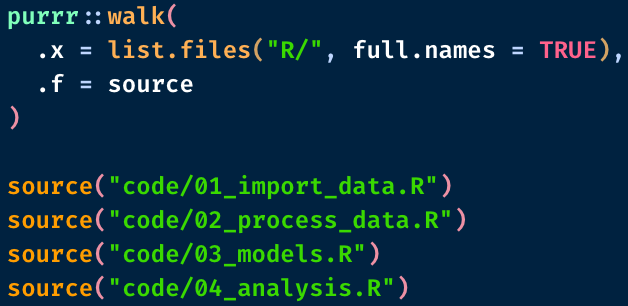
\includegraphics[width = 0.7\textwidth]{code.png}
    \end{figure}
    \begin{exampleblock}{Idée}
        \begin{itemize}
            \fleche Centralisation des fonctions dans le dossier \texttt{R}
        \end{itemize}
    \end{exampleblock} 
    \begin{alertblock}{Problèmes}
        \begin{itemize}
            \fleche Si on fait un changement quelque part, qu'est-ce qu'il faut rerouler?
            \fleche Est-ce que tout est bien synchronisé (i.e. à jour)?
        \end{itemize}
    \end{alertblock} 
\end{column}
\end{columns}

\end{frame}
% ----------------------------

\begin{frame}[t]{Organisation d'un projet de science des données}

\Large \textbf{Option \#3, avec \texttt{targets}}

\small

\begin{columns}[T] % align columns
\begin{column}{.25\textwidth}
    \begin{forest}
        for tree={
            font=\ttfamily,
            grow'=0,
            child anchor=west,
            parent anchor=south,
            s sep = 1pt,
            anchor=west,
            calign=first,
            edge path={
                \noexpand\path [draw, \forestoption{edge}]
                (!u.south west) +(7.5pt,0) |- node[fill,inner sep=1.25pt] {} (.child anchor)\forestoption{edge label};
            },
            before typesetting nodes={
            if n=1
            {insert before={[,phantom]}}
            {}
        },
        fit=band,
        before computing xy={l=15pt},
      }
        [dossier projet
          [R
            [utils.R]
            [get\_data.R]
            [transform\_data.R]
            [fit\_model.R]
          ]
          [\_targets
            [meta]
            [objects]
          ]
          [data
            [claims.csv]
            [contracts.csv]
          ]
        [ad\_hoc
            [test\_glm\_models.R]
          ]
          [project.Rproj]
          [\jaune{targets.R}]
        ]
    \end{forest}
\end{column}
\hfill
\begin{column}{.64\textwidth}
   Définition du pipeline dans \texttt{\_targets.R}
   \begin{figure}
       \flushleft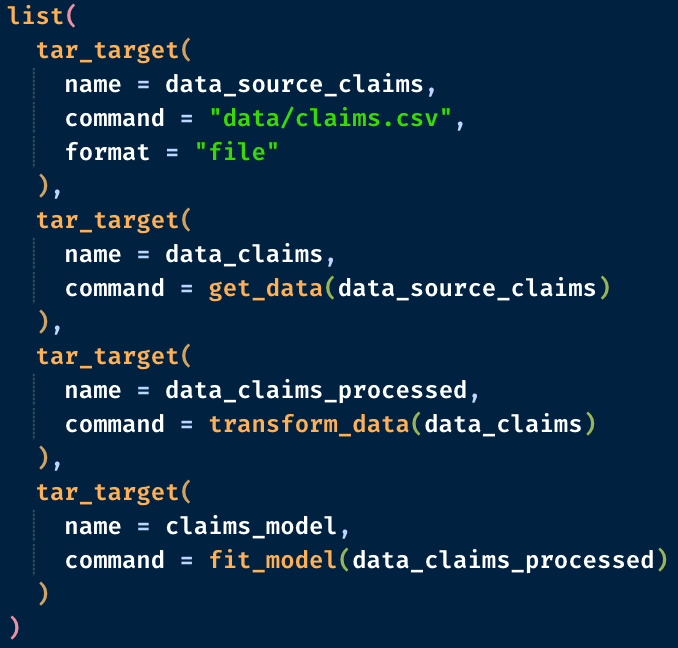
\includegraphics[width = 0.8\textwidth]{code_2.png}
   \end{figure}
\end{column}
\end{columns}

\end{frame}

% ----------------------------

\begin{frame}{Démarrer un nouveau projet \texttt{targets}}

\begin{itemize}
    \item[$\circled{0}$] Installer le package: \texttt{install.packages("targets")}
    \item[$\circled{1}$] Créer un nouveau projet \texttt{R}
    \item[$\circled{2}$] Enregistrer un fichier (vide) appelé \texttt{\_targets.R} dans le dossier de projet
    \item[$\circled{3}$] Créer 2 nouveaux dossiers: \texttt{data} et \texttt{R} (recommandé)
\end{itemize}

\vspace{1cm}
\begin{forest}
    for tree={
        font=\ttfamily,
        grow'=0,
        child anchor=west,
        parent anchor=south,
        s sep = 1pt,
        anchor=west,
        calign=first,
        edge path={
                \noexpand\path [draw, \forestoption{edge}]
                (!u.south west) +(7.5pt,0) |- node[fill,inner sep=1.25pt] {} (.child anchor)\forestoption{edge label};
        },
        before typesetting nodes={
        if n=1
        {insert before={[,phantom]}}
        {}
    },
    fit=band,
    before computing xy={l=15pt},
  }
    [dossier projet
        [nom\_du\_projet.Rproj]
        [\_targets.R]
        [data]
        [R]
    ]
\end{forest}
    
\end{frame}

% ----------------------------

\begin{frame}{Fichier \texttt{\_targets.R}}
    
Dans le script \texttt{\_targets.R} vous devez:
\begin{itemize}
    \item[$\circled{1}$] Importer le package: \texttt{library(targets)}
    \item[$\circled{2}$] Importer vos fonctions personnelles (qui sont dans le dossier \texttt{R})
    \item[$\circled{3}$] Appeller la fonction \texttt{tar\_option\_set()} si vous souhaitez modifier les comportements par défaut
    \item[$\circled{4}$] Définir vos \og{}targets\fg{} avec la fonction \texttt{tar\_target}. Un target est simplement une étape de votre pipeline. C'est un \motcle{objet d'intérêt} dans votre projet. Ça peut être n'importe quel objet \texttt{R}: un jeu de données, un graphique, un modèle ajusté, les résultats d'une analyse, etc. Au minimum, un target doit avoir un nom et une commande \texttt{R}. Lorsque le pipeline sera exécuté, un dossier \texttt{\_target/objects} sera créé, dans lequel les objets sont stockés.
    \item[$\circled{5}$] Le script doit se terminer par une liste (dans n'importe quel ordre) de vos targets
\end{itemize}
    
\end{frame}

% ----------------------------

\begin{frame}[t]{Exemple minimal}

\begin{columns}[T] % align columns
\begin{column}{.25\textwidth}
    \begin{forest}
    for tree={
        font=\ttfamily,
        grow'=0,
        child anchor=west,
        parent anchor=south,
        s sep = 1pt,
        anchor=west,
        calign=first,
        edge path={
                \noexpand\path [draw, \forestoption{edge}]
                (!u.south west) +(7.5pt,0) |- node[fill,inner sep=1.25pt] {} (.child anchor)\forestoption{edge label};
        },
        before typesetting nodes={
        if n=1
        {insert before={[,phantom]}}
        {}
    },
    fit=band,
    before computing xy={l=15pt},
  }
    [.
        [exemple\_minimal.Rproj]
        [\_targets.R]
        [data
            [boston.csv]
        ]
        [R
            [make\_scatter\_plot.R]
        ]
    ]
\end{forest}
\end{column}
\hfill
\begin{column}{.55\textwidth}
    \large Fichier \texttt{make\_scatter\_plot.R}:
    \vspace{-0.2cm}
    \begin{figure}
        \flushleft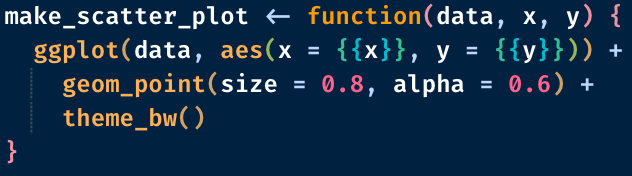
\includegraphics[width = 0.9\textwidth]{exemple_minimal_2.png}
    \end{figure}
\end{column}
\end{columns}

\large Fichier \texttt{\_targets.R}:
\vspace{-0.2cm}
\begin{figure}
    \flushleft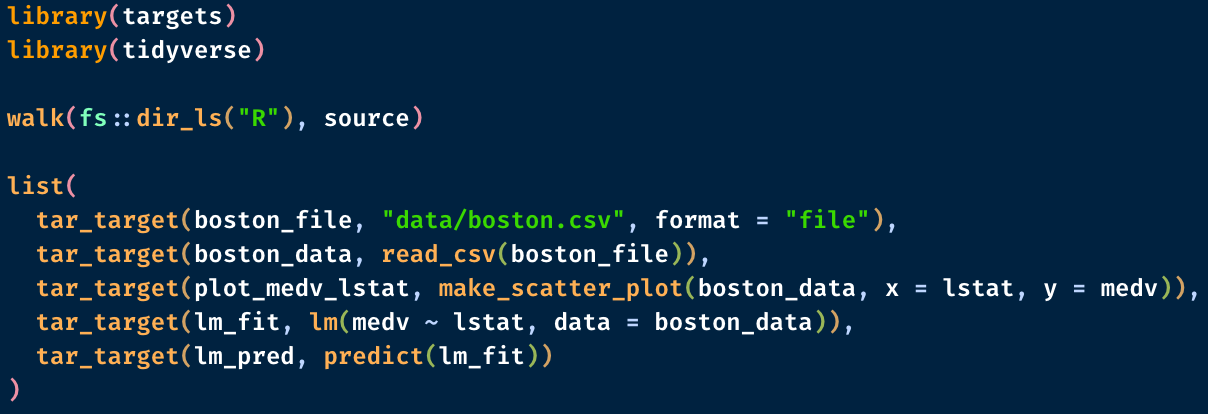
\includegraphics[width = 0.9\textwidth]{exemple_minimal_1.png}
\end{figure}

\url{https://github.com/francisduval/minimal_example_targets}

\end{frame}

% ----------------------------

\begin{frame}{Exemple minimal}

\large \textbf{Fonctions populaires du package \texttt{targets}}

\normalsize
\begin{table}
    \centering
    \begin{tabular}{l p{5cm} c}
        \toprule
        \textbf{Fonction} & \textbf{Utilité} & \textbf{Habituellement utilisée dans}\\
        \midrule
        \rowcolor{grispale}\texttt{tar\_target} & définir les targets & \texttt{\_targets.R}\\
        \texttt{tar\_make} & exécuter le pipeline & console \texttt{R}\\
         \rowcolor{grispale}\texttt{tar\_visnetwork} & visualiser le pipeline & console \texttt{R}\\
         \texttt{tar\_manifest} & renvoie une base de données qui décrit le pipeline & console \texttt{R}\\
         \rowcolor{grispale}\texttt{tar\_option\_set} & définir les options & \texttt{\_targets.R}\\
        \texttt{tar\_read} & lire les targets & console \texttt{R}\\
         \rowcolor{grispale}\texttt{tar\_prune} & supprimer les objets dans \texttt{\_targets/objects} qui ne font plus partie du pipeline & console \texttt{R}\\
        \texttt{tar\_destroy} & supprimer tous les objets (ou une partie des objets, si spécifié en argument) dans \texttt{\_targets/objects} & console \texttt{R}\\
    \end{tabular}
\end{table}

\end{frame}

% ----------------------------

\begin{frame}{Exemple minimal -- Exercice}

\begin{itemize}
    \item[$\circled{1}$] Télécharger le dépôt sur GitHub et ouvrir le projet \texttt{R} sur RStudio
    \item[$\circled{2}$] Ouvrir le script \texttt{\_targets.R}. Importer les packages
    \item[$\circled{3}$] Visualiser le pipeline avec \texttt{tar\_visnetwork()}
    \begin{itemize}
        \fleche Tout est \og{}outdated\fg{} car le pipeline n'a pas encore été exécuté
    \end{itemize}
    \item[$\circled{4}$] Exécuter le pipeline avec \texttt{tar\_make()}
    \begin{itemize}
        \fleche Observer qu'un nouveau dossier \texttt{\_targets} a été créé
    \end{itemize}
    \item[$\circled{5}$] Visualiser de nouveau le pipeline avec \texttt{tar\_visnetwork()}
    \begin{itemize}
        \fleche Tout est maintenant à jour
    \end{itemize}
    \item[$\circled{6}$] Faire une modification de votre choix dans la fonction \texttt{make\_scatter\_plot}
    \item[$\circled{7}$] Visualiser de nouveau le pipeline avec \texttt{tar\_visnetwork()}
    \begin{itemize}
        \fleche Tous les targets qui dépendent de cette fonction sont maintenant \og{}outdated\fg{}
    \end{itemize}
    \item[$\circled{8}$] Exécuter le pipeline de nouveau avec \texttt{tar\_make()}
    \item[$\circled{9}$] Visualiser de nouveau le pipeline avec \texttt{tar\_visnetwork()} et observer que tout est redevenu à jour
    \item[$\circled{10}$] Lire un des targets avec la fonction \texttt{tar\_read}
    \item[$\circled{11}$] Ajouter un target de votre choix qui dépend d'un ou plusieurs autres targets existants. Visualiser le pipeline. Exécuter le pipeline.
\end{itemize}


\end{frame}

% ----------------------------

\begin{frame}{Suivre les modifications de fichiers externes}

\begin{itemize}
    \fleche Si votre pipeline importe un \motcle{fichier de données préexistant} ou crée des fichiers en dehors dossier ``\texttt{\_targets/objects}'', il est recommandé de surveiller leurs modifications
    \fleche De cette façon, \texttt{tar\_make()} va mettre à jour automatiquement les targets en aval si ces fichiers changent.
\end{itemize}


\begin{exampleblock}{Exemple pour fichier de données externe}
    Recommandé:
    \begin{figure}
        \centering
        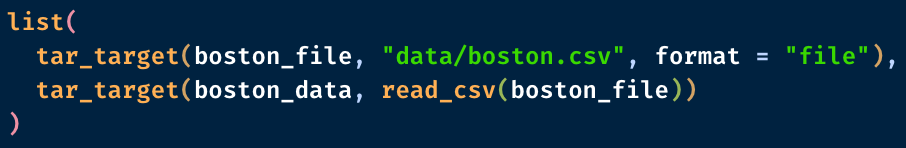
\includegraphics[width = 0.9\textwidth]{fichier_externe_2.png}
    \end{figure}
    Non recommandé:
    \begin{figure}
        \centering
        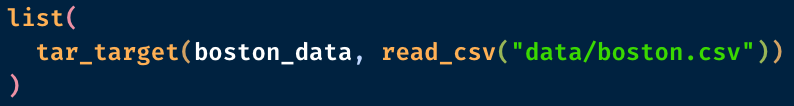
\includegraphics[width = 0.9\textwidth]{fichier_externe_1.png}
    \end{figure}
\end{exampleblock}

\end{frame}

% ----------------------------

\begin{frame}{Suivre les modifications de fichiers externes}

\textbf{Exporter des graphiques}

\begin{itemize}
    \fleche Le target suivant va produire un graphique et le stocker dans le magasin de données "\texttt{\_targets/objects}":
    \begin{figure}
        \centering
        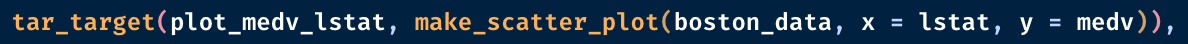
\includegraphics[width = 0.9\textwidth]{export_graphique_1.png}
    \end{figure}
    \fleche On peut vouloir à la place exporter ce graphique en format .PNG: 
    \begin{figure}
        \centering
        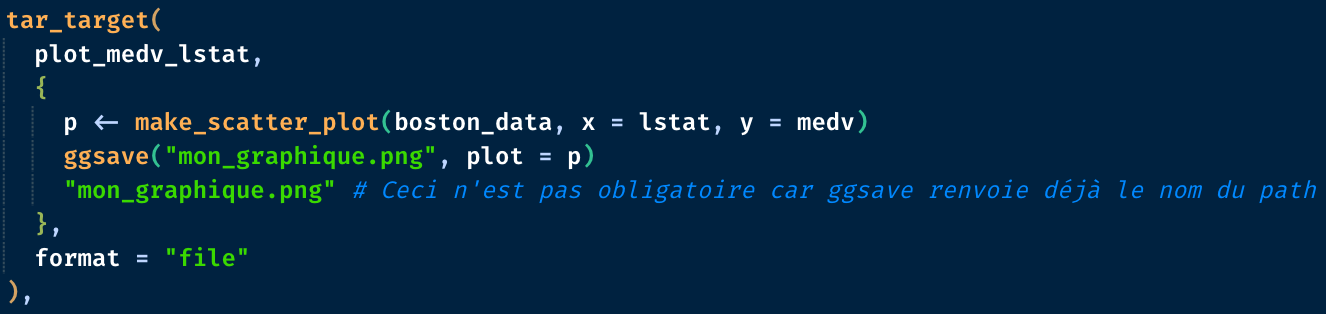
\includegraphics[width = 0.9\textwidth]{export_graphique_2.png}
    \end{figure}
    \fleche \og{}\texttt{format = "file"}\fg{} permet de suivre les modifications faites à l'adresse ``\texttt{mon\_graphique.png}''.
\end{itemize}

\end{frame}

% ----------------------------

\begin{frame}{Targets de type \og{}pattern\fg{}}

\textbf{Considérer l'exemple minimal}
\begin{itemize}
    \fleche On a un target qui ajuste une régression linéaire simple avec \texttt{lstat} comme variable explicative
    \fleche On veut maintenant ajuster une régression linéaire simple pour chacune des variables explicatives \texttt{lstat}, \texttt{crim} et \texttt{zn}
    \fleche On se définit d'abord une fonction qui ajuste une régression linéaire simple:
    \begin{figure}
        \centering
        \flushleft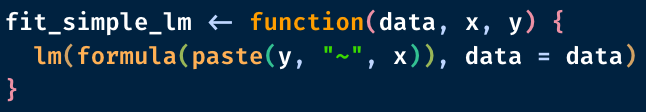
\includegraphics[width = 0.5\textwidth]{fonction_lm.png}
    \end{figure}
    \fleche Ensuite, on définit le target des variables explicatives:
    \begin{figure}
        \centering
        \flushleft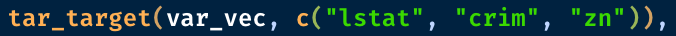
\includegraphics[width = 0.5\textwidth]{var_vec.png}
    \end{figure}
    \fleche Finalement, on ajuste les régressions linéaires et on les stocke dans une liste:
    \begin{figure}
        \centering
        \flushleft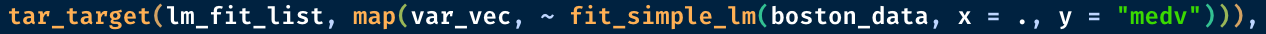
\includegraphics[width = 0.9\textwidth]{lm_fit_list.png}
    \end{figure}
    \fleche Problème: si on ajoute un élément à \texttt{var\_vec}, tout sera re-roulé (c'est problématique si le target \texttt{lm\_fit\_list} est long à rouler)
\end{itemize}

\end{frame}

% ----------------------------

\begin{frame}{Targets de type \og{}pattern\fg{}}

\begin{itemize}
    \fleche Une meilleure alternative est de créer un target de type \og{}pattern\fg{}:
    \begin{figure}
        \centering
        \flushleft
\includegraphics[width = 0.93\textwidth]{lm_fit_pattern.png}
    \end{figure}
    \fleche \texttt{targets} va alors créer un target possédant plusieurs \og{}branches\fg{}. 
    \fleche Cette manière de procéder est appelée \motcle{dynamic branching}
\end{itemize}

\textbf{Exercice:}

\begin{itemize}
    \item[$\circled{1}$] Ajouter le target \texttt{var\_vec} ainsi que le pattern \texttt{lm\_fit\_pattern} à votre pipeline
    \item[$\circled{2}$] Rouler le pipeline et l'examiner avec \texttt{tar\_visnetwork}
    \item[$\circled{3}$] Importer le target \texttt{lm\_fit\_pattern} dans l'environnement global avec \texttt{tar\_read} et l'examiner
    \item[$\circled{4}$] Ajouter une variable au target \texttt{var\_vec}
    \item[$\circled{5}$] Visualiser le pipeline
    \item[$\circled{6}$] Rouler le pipeline de nouveau. Observer que \texttt{targets} va sauter les branches qui ont déjà été roulées
\end{itemize}

\textbf{Défi pour après la présentation:}
\begin{itemize}
    \fleche Définir un target de type \og{}pattern\fg{} qui prend en entrée le pattern \texttt{lm\_fit\_pattern} (entre autres) et qui renvoie un pattern contenant le nuage de points et la droite de régression pour chacune des régressions
\end{itemize}

\end{frame}

% ----------------------------

\begin{frame}{Fichier RMarkdown en tant que target}

\begin{itemize}
    \fleche Il est possible avec la fonction \texttt{tarchetypes::tar\_render()} d'ajouter un \motcle{rapport RMarkdown} à votre pipeline
    \fleche Votre rapport devrait \motcle{s'exécuter rapidement}: les gros calculs devraient être faits dans les autres targets
\end{itemize}

\textbf{Intégrer un rapport RMarkdown à votre pipeline:}

\begin{itemize}
    \item[$\circled{1}$] Écrire votre rapport dans un fichier \texttt{.Rmd}. Celui-ci devrait importer des targets avec la fonction \texttt{tar\_read()}. Le sauvegarder dans le répertoire
    \item[$\circled{2}$] Ajouter le target du rapport à votre pipeline avec \texttt{tarchetypes::tar\_render()}:
    \begin{figure}
        \centering
        \flushleft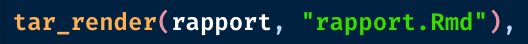
\includegraphics[width = 0.4\textwidth]{tar_render.png}
    \end{figure}
    \item[$\circled{3}$] Appeler \texttt{tar\_visnetwork()} pour voir si le rapport est bel et bien intégré
    \item[$\circled{4}$] Rouler le pipeline et observer que votre rapport (en format .html ou .pdf) est apparu dans le répertoire
\end{itemize}

\end{frame}

% ----------------------------

\begin{frame}{Options}
    
\begin{itemize}
    \fleche Il est possible d'écraser plusieurs comportements par défaut avec la fonction \texttt{tar\_option\_set}
    \fleche À mettre au début du script \texttt{\_targets.R}:
    \begin{figure}
        \centering
        \flushleft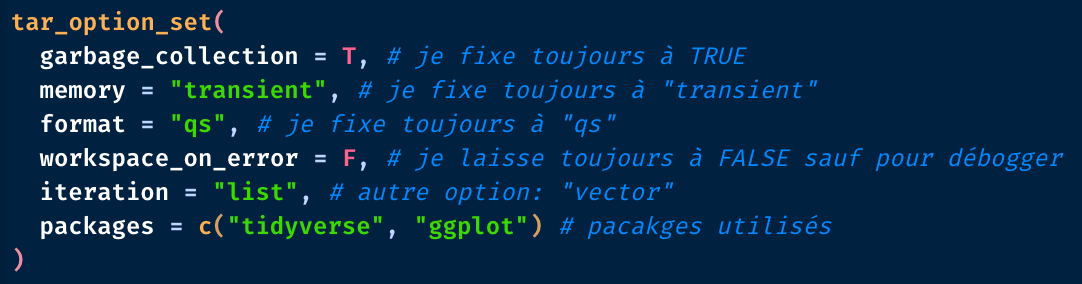
\includegraphics[width = 0.75\textwidth]{tar_option_set.png}
    \end{figure}
    \fleche Certaines options peuvent être changées dans chaque target de manière individuelle
\end{itemize}

\end{frame}

% ----------------------------

\begin{frame}{Vive les fonctions!}

\begin{block}{3 bénéfices de créer des fonctions}
    \begin{itemize}
        \fleche Meilleure abstraction du code
        \fleche Pas de duplication du code (on peut réutiliser les fonctions)
        \fleche Le fichier \texttt{\_targets.R} est plus facile à lire et moins long avec des fonctions
    \end{itemize}
\end{block}

\textbf{Recommandé:}
\begin{figure}
    \centering
    \flushleft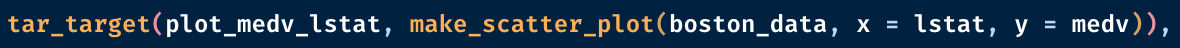
\includegraphics[width = 0.9\textwidth]{exemple_2.png}
\end{figure}

\textbf{Non recommandé:}
\begin{figure}
    \centering
    \flushleft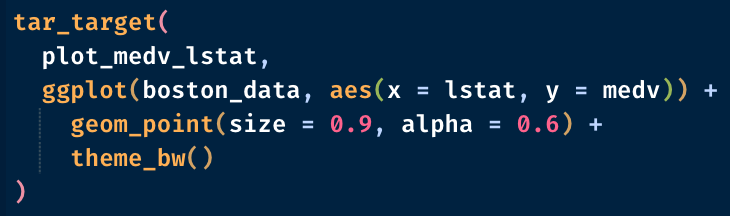
\includegraphics[width = 0.7\textwidth]{exemple_1.png}
\end{figure}

\end{frame}

% ----------------------------

\begin{frame}{Quelques trucs utiles}
    
\textbf{Plus de détails avec \texttt{tar\_visnetwork}}
\begin{figure}
    \centering
    \flushleft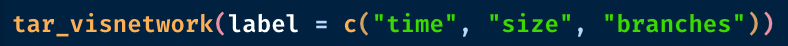
\includegraphics[width = 0.7\textwidth]{tar_vis_code.png}
\end{figure}

\begin{figure}
    \centering
    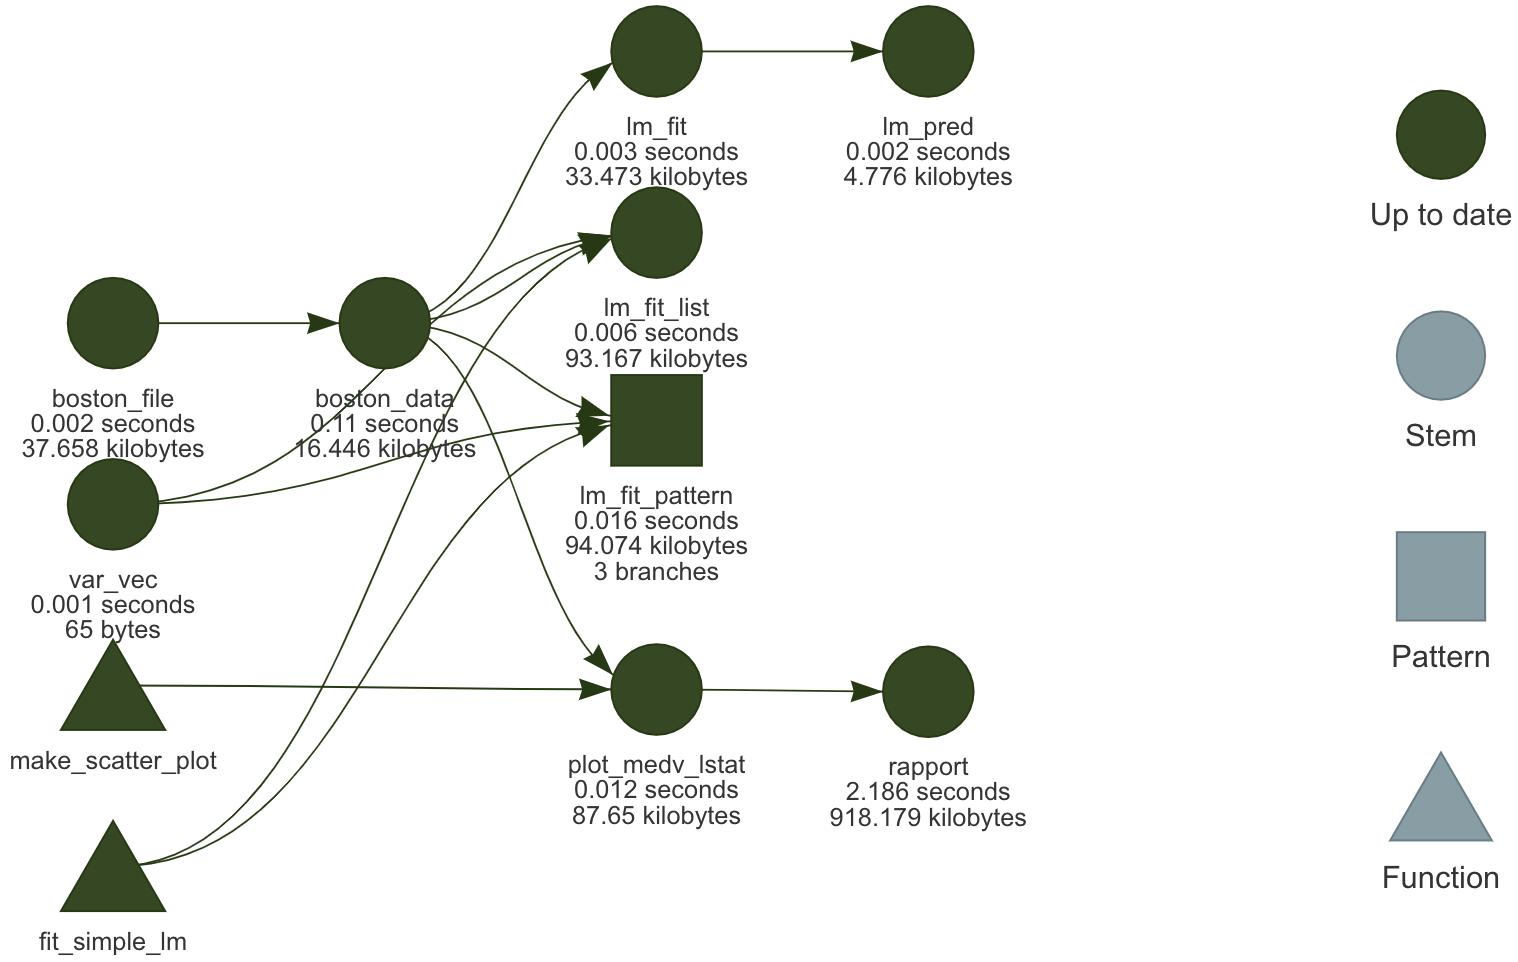
\includegraphics[width = 0.9\textwidth]{tar_visnetwork_options.png}
\end{figure}

\end{frame}

% ----------------------------

\begin{frame}{Quelques trucs utiles}

\textbf{Empêcher un target de s'exécuter}
\begin{figure}
    \centering
    \flushleft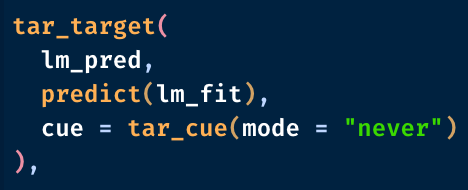
\includegraphics[width = 0.5\textwidth]{tar_cue.png}
\end{figure}


\end{frame}

% ----------------------------

\begin{frame}{Liens utiles}
    
\begin{itemize}
    \fleche \textbf{Présentation du package par Will Landau:}
    \begin{itemize}
        \blt \url{https://www.youtube.com/watch?v=Gqn7Xn4d5NI&t}
    \end{itemize}
    \fleche \textbf{Excellent tutoriel d'une demi-journée créé par Will Landau (demande d'avoir un compte RStudio Cloud):}
    \begin{itemize}
        \blt \url{https://rstudio.cloud/project/1699460}
    \end{itemize}
    \fleche \textbf{Manuel de l'utilisateur du package:}
    \begin{itemize}
        \blt \url{https://books.ropensci.org/targets/}
    \end{itemize}
\end{itemize}
    
\end{frame}

% ----------------------------

\begin{frame}{Exercice}
    
Sélectionnez un jeu de données quelconque. Construire un pipeline de science des données à partir de ce jeu de données. Votre projet devra:

\begin{itemize}
    \fleche suivre les modifications du jeu de données choisi (en utilisant \og{}\texttt{format = "file"}\fg{}),
    \fleche contenir un target qui exporte un ou plusieurs graphique(s) dans un dossier nommé \og{}figures\fg{} (que vous devez créer),
    \fleche contenir au moins un target de type \og{}pattern\fg{},
    \fleche contenir un target qui suit les modifications d'un rapport RMarkdown. Vous devez préalablement créer ce rapport, que vous sauvegarderez dans un dossier nommé \og{}reports\fg{}. 
\end{itemize}
    
\end{frame}

% ------------------------------------------------------------------------------------------------------------------------------

\end{document}